\chapter{Konzeption}
\label{chap:konzept}
    In diesem Kapitel wird das erarbeitete Konzept dargelegt. Basierend auf den 
    Anforderungen, die aus den Anwendungsfällen, den Experteninterviews und der Zielgruppenanalyse 
    erhoben wurden, werden die daraus generierten Überlegungen und Entscheidungen transparent 
    dargestellt. Durch die bereits erfolgte Anforderungsanalyse (siehe Kapitel \ref{chap:anforderungsanalyse})
    sind erste Schritte der Konzeption abgeschlossen. 
    \\
    Zu Anfang des Kapitels wird das allgemeine Ziel eines Konzeptes, sowie die konkrete Absicht hinter dieser Arbeit 
    erläutert. Anschließend 
    wird auf das Anwendungsumfeld des Systems (\ref{sec:anwendungsumfeld}) eingegangen, darunter die
    zusätzlichen Komponenten, die notwendig sind, um das Framework in einer dafür vorgesehenen Umgebung sinnvoll 
    einzusetzen. Darauffolgend wird anhand der zugrundeliegenden Informationen und Anforderungen das 
    Architekturkonzept (\ref{sec:architekturkonzept}) ausgeführt. 
    Dabei wird auf verschiedene kontextabhängige Aspekte, sowie auf die Sichtweisen des Anwenders und des Frameworks eingegangen.


\section{Ziel der Konzeption}
\label{sec:konzeptziele}
    Das Ziel einer Konzeption ist die Veranschaulichung von abstrakten Ideen und Entwürfen. %und Leitideen. 
    Hierbei werden aus den zugrundeliegenden Problemstellungen, Szenarien und Anforderungen Entwürfe und 
    Lösungsmöglichkeiten erarbeitet und identifiziert. Diese helfen bei der Aufstellung von notwendigen Schritten 
    und dienen als Grundlage zur Untermauerung und Darlegung von Entscheidungen. Somit wird Dritten der Kontext, die 
    Domäne und das zu lösende Problem, bzw. die Lösung dargestellt. 
    \\
    \linebreak
    Das Konzept dieser Thesis 
    erarbeitet eine Lösung zur Implementierung einer Anwendung, die es ermöglicht, Automatisierungen, Regeln und Prozesse innerhalb eines 
    Firmenbüros zu koordinieren. Der Fokus liegt dabei verstärkt auf der einfachen Nutzung des Frameworks für den Anwender und 
    die uneingeschränkte und schnell umzusetzende Ausprägungsvielfalt von Regelprozessen. Dadurch kann der Anwender die vorgegebene Struktur nutzen, um individuelle 
    Sachverhalte zu realisieren, die in seinem Umfeld abzudecken sind. Im Rahmen dieser Arbeit werden verstärkt Anwendungsfälle mit einem Service-Roboter 
    umgesetzt.
    %\\
    Hierfür wird der allgemeine Aufbau der Architektur skizziert und demonstriert, wie eine solche Lösung aussehen kann. 
    Unter Berücksichtigung der Forschungsfrage (siehe Abschnitt \ref{sec:forschungsfragen}) wird eine Möglichkeit offengelegt, mit der 
    ein Softwareentwickler neue Regeln entwickeln und dem System hinzufügen kann, ohne ein weiteres zu erlernendes Framework zu verwenden. 
    Dabei sollen die notwendigen Schritte und Interaktionen formalisiert und für den Entwickler vereinfacht werden. 
    %\\
    %\linebreak
    %In folgender Darlegung wird nochmals konkreter auf den Kontext als auch auf die Intension der Arbeit eingegangen. 
    % Das Ziel des Konzeptes ist es, dem Entwickler den Aufwand zur Erweiterung des Systems zu minimieren durch weitere 
    % Regeln und Abdeckung von Anwendungsfällen (Use Cases) und eine Struktur vorgeben. (ToDo's, Flexibilität in der 
    % Umsetzung (nicht wie Home Assistant und openHAB eher eingeschränkt)) 

%\section{Abzudeckende Funktionalitäten}
%\label{sec:konzeptfunktionalitaet}
    % Was soll der Entwickler machen können? 
    % Welche Grundlagen braucht er, um eine Regel implementieren zu können?
    % Welche Funktionen müssen gegeben sein, um die Struktur vorzugeben? 
    % Reicht ein Hinweis weöche Stellen angepackt werden müssen, um eine Regel hinzuzufügen? 
    
    %%%%%%%%%%%%%%%%%%%%%%%%%%%%%%%%%%%%%%%%%%%%%%%%%%%%%%%%%%%%%

    % ZIEL DES KONZEPTES: Ein Framework für Entwickler bereitzustellen, welches die Mächtigkeit für den Entwickler offen lässt, nicht einschränkt 
    % und dennoch Konfiguration und Ausführung umsetzt. Der Entwickler muss lediglich den Zustandsraum, die MQTT-Topics und die Regeln definieren.
    % Der Entwickler bekommt ein Framework an die Hand, welches die Umsetzung von Prozessen in einem smarten Büro ermöglicht. Das Framework kümmert sich um die 
    % Organisation und die Ausführung der Regeln. Die Richtigkeit der Regeln und des Zustandsraumes muss der Entwickler sicherstellen. 
    % Die Kommunikation über MQTT ist nur eine Möglichkeit. Das Setup wird wegabstrahiert 

    %%%%%%%%%%%%%%%%%%%%%%%%%%%%%%%%%%%%%%%%%%%%%%%%%%%%%%%%%%%%%

\section{Anwendungsumfeld}
\label{sec:anwendungsumfeld}
    Grundsätzlich ist der Einsatzort des Frameworks variabel, da die eigentliche Implementierung und Nutzung der Regeln und Prozesse 
    abhängig vom Anwender und dessen Umfeld sind. Dadurch kann sowohl im privaten \acl{SH} Umfeld als auch in Büroräumen ein System mithilfe des 
    Frameworks aufgebaut werden. Basierend auf den vorangestellten Tätigkeiten, darunter die Anforderungsanalyse, und der Eingrenzung auf den 
    Einsatz im Smart Office liegt darauf der Fokus. % Schwerpunkt der Arbeit auf dem Einsatz in einem smarten Büro. 
    \\
    \linebreak
    Stützend auf den vorab ermittelten Anwendungsfällen (siehe Abschnitt \ref{subsec:checkin} und \ref{subsec:evacuation}) sind unabhängige 
    Komponenten, darunter bspw. ein Service-Roboter und weitere einsatzfähige Geräte, sowie ein \acs{MQTT}-Broker notwendig. Ein \acs{MQTT}-Broker 
    wird im Zuge der Konzeption von dem Framework selbst nicht bereitgestellt, lediglich die Client-Anbindung wird gegeben. Der Anwender muss sich selbstständig um den verfügbaren Broker kümmern. 
    Dadurch kann die Anforderung einer Kommunikation mittels \acs{MQTT} umgesetzt werden. Eine denkbare infrastrukturelle 
    Architektur kann wie folgt aussehen: 
    \begin{figure}[hbt!]
        \centering
        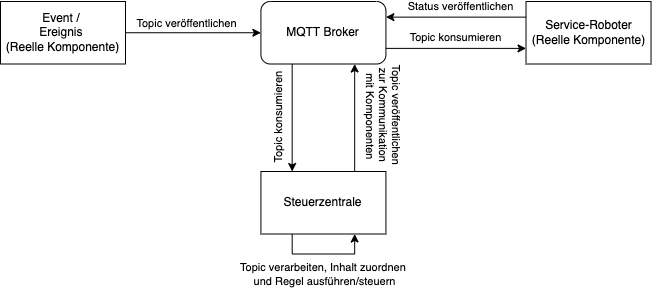
\includegraphics[width=14cm,height=11cm,keepaspectratio]{images/Systemarchitektur.png}
        \caption{Infrastruktur des Anwendungsumfeldes der Steuerzentrale}
        \label{fig:infrastructure}
    \end{figure}

\section{Konzept}
\label{sec:concept}
    Die Intension, die hinter der Ausarbeitung dieses Konzeptes steht, ist zum einen die einfache Handhabung der 
    formalisierten Interaktionen für Softwareentwickler %während
    unter der Verwendung des Frameworks und zum anderen die 
    offene Gestaltung von Regelprozessen. Dadurch ist der Anwender bei der Implementierung von Regeln, Aufgaben und Automatisierungen 
    für ein intelligentes Büro nicht eingeschränkt und kann mit der Regeldefinition flexibel variieren.
    %einzugrenzen zu beschränken. 
    Es soll lediglich ein Muster vorgegeben werden, damit Regeln einheitlich als solche von dem Framework 
    verarbeitet und genutzt werden können. 
    \\ 
    \linebreak
    Bei vergleichbaren Softwareprodukten, die im Rahmen dieser Arbeit erläutert 
    wurden (siehe Kapitel \ref{sec:homeassistant} und \ref{sec:openhab}), ist die Vielfalt der Regelausprägung auf 
    den Kontext des Systems eingeschränkt und benötigt mehrere Schritte, um sie zu realisieren. Dies bedeutet, dass 
    Regeln und Prozesse nur mit Komponenten und Informationen innerhalb des Systems arbeiten können, bzw. benötigte 
    Informationen erst durch eine systemseitige Erweiterung durch Plugins verfügbar sind, auf die der Nutzer keinen direkten 
    Einfluss nehmen kann. Mit den bestehenden Lösungen wird versucht, die Regeldefinition für Endnutzer so 
    einfach wie möglich zu gestalten, wodurch eventuell erst zahlreiche Selektionen über die Benutzeroberfläche zum gewünschten Ziel führen.   
    \\
    \linebreak
    Um dennoch dem Anwender eine Struktur vorzugeben, mit der Regeln definiert und zur Laufzeit der Anwendung ausgeführt 
    werden können, soll mit diesem Konzept ein Framework zum Lösen dieser Herausforderungen erarbeitet werden. Hierfür soll 
    der Anwender mit der Komplexität der Regelverwaltung und deren Durchführung nicht konfrontiert werden. Dieser ist lediglich 
    in der Verantwortung, die für ihn notwendigen Regeln und Prozesse zu definieren und dem Framework bereitzustellen. 
    Dadurch soll dem Framework-Verwender die Möglichkeit geboten werden, das zur Verfügung gestellte System 
    mit individuellen Regeln, dafür vorgesehenen Bedingungen, Komponenten und deren Zustände zu implementieren. Beispielsweise 
    können bei Regeldefinitionen Informationen direkt von Datenpunkten über \acs{HTTP}-Abfragen bezogen werden, bzw. Ressourcen 
    und Inhalte individuell nachgezogen werden.
    \\ 
    Das Konzept beinhaltet die in folgendem Abschnitt dargelegten grundsätzlichen Komponenten. %Aus denen bildet sich der grundlegende Aufbau 
    %des Frameworks.

    \subsection{Konzeptkomponenten}
    \label{subsec:conceptcomps}
        Für die Erläuterung des Konzeptes werden vorab die einzelnen Konzeptkomponenten dargelegt, da diese die Anhaltspunkte 
        für den weiteren Verlauf und den Kern des Frameworks darstellen: % . Das Framework baut auf folgenden Bausteinen auf:
        \begin{itemize} 
            \item Regel (Rule): Eine Regel ist ein Konstrukt, welches bei bestimmten Events die darin enthaltenen Aktionen ausführen soll. 
            Der grobe Aufbau einer Regel ist immer gleich. Diese beinhaltet einen Auslöser, eine Bedingung, einen Prozess und einen eindeutigen 
            Namen. Die Inhalte der Regel kann der Anwender ja nach Bedarf beliebig ausprägen und ergänzen. 
            \item Komponente (Component): Eine Komponente soll einen reellen Gegenstand abbilden, der bei Benutzung durch eine Regel unter anderem 
            für weitere gesperrt und danach freigegeben werden kann. Diese Komponente kann ebenso sämtliche Zustände beinhalten und als Objekt in den Zustandsraum aufgenommen werden.
            \item Zustandsraum (State): Der Zustandsraum, das sog. Zustandsobjekt, soll alle Zustände von Komponenten und weiteren Geräten abbilden. Dieser repräsentiert die Zustände der Realität.
            \item Auslöser (Trigger): Ein Auslöser löst im Allgemeinen eine Zustandsänderung aus. Im Kontext des Frameworks gibt es zwei Ausprägungen von 
            Auslösern. Zum einen werden eingehende Aktionen entgegengenommen und über die Transformation zu einer Zustandsänderung verarbeitet, zum anderen können durch Regelprozesse 
            wiederum weitere Schritte und Zustandsänderungen ausgelöst werden. Dadurch werden ausgehende Aktionen gesteuert. 
            %Der Auslöser ist unter anderem ein von außen einwirkendes Objekt, das Zustandsänderungen hervorruft. Beispielsweise ist ein 
            %Auslöser das eintreffen eines Events über eine Kommunikationsschnittstelle. Ebenso können durch Regelprozesse Events ausgelöst werden. 
            \item Transformation (Transformer): Mit der Transformation werden eingehenden Zustandsänderungen, die durch ein Event oder Auslöser ausgelöst werden, 
            auf das eigentliche Zustandsobjekt übertragen. 
            %, die eine Zustandsänderung bewirken, die durch einen Auslöser hervorgerufen 
            %werden und eine Zustandsänderung bewirken
        \end{itemize}
        %Diese Komponenten bilden den Kern des Frameworks.
        %In folgendem Abschnitt wird nochmals auf die Sichten eingegangen und anhand denen der Ablauf des Frameworks als auch die 
        %Aufgaben des Anwenders erläutert. %Der Ablauf des Prozesses von Auslöser bis zur Ausführung der Regel wird anhand eines Programmablaufdiagramms gestützt.
        %\\
        %\linebreak
        Das Konzept wird aus zweierlei Sichtweisen betrachtet, die in folgendem Abschnitt aufgegriffen werden und für die weitere 
        Konzepterläuterung notwendig sind.
    
    \subsection{Sichtweisen}
    \label{subsec:sichtweisen}
        Wie bereits aus dem Kontext hervorgeht, wird das System aus zwei Perspektiven beleuchtet. Zum einen aus Sicht des Anwenders, 
        der das Aufsetzen und in Betrieb nehmen des Systems, sowie das Definieren und Implementieren von Regeln als 
        Aufgabe übernimmt. Zum anderen die 
        Bereitstellungssicht, die das Framework als ausführende Kraft besetzt. Dieses sorgt für die Erfüllung der vom 
        Anwender definierten Regeln. Ebenso stellt es Funktionen bereit, die das Empfangen von Events, das Starten 
        von Regeln und Prozessen ermöglicht. Das Management dazu wird vom Framework übernommen. 
        Das Konzept widmet sich grundlegend dem initialen Aufbau des Frameworks. 
        \\
        \linebreak
        Der Anwender hat das initiale Setup des Frameworks zur Aufgabe. Zuerst sollte der Zustandsraum erstellt werden. 
        Darin sind alle notwendigen Zustände als Attribute und Objektfelder abzubilden. Diese können konkret Geräte sein, die im Rahmen des 
        intelligenten Büros verwendet werden, bspw. ein Service-Roboter, ein Türöffner und weitere steuerbare Geräte, die 
        ihren Zustand ändern können. Nachdem das Zustandsobjekt 
        definiert wurde, geht es in die Implementierung der Regeln. Diese sind individuell je nach 
        Anforderungen des Anwenders zu erstellen. Jedoch sind bestimmte Funktionen und Vorgaben bezüglich Bedingungsprüfung 
        und Regeldurchlauf einzuhalten. Anforderungen dabei sind das Implementieren von drei unabdingbaren Funktionen. 
        Die erste Funktion ist die Zuordnung des Auslösers, der bei einem bestimmten Event eine Regel durchläuft. 
        Die zweite zu implementierende Funktion ist die Prüfung von Werten im Zustandsraum, sodass beim Eintreten spezifischer 
        Bedingungen und Zuständen bestimmte Regelprozesse ausgeführt werden können. Die dritte vorgegebene Funktion ist die 
        des eigentlichen Regeldurchlaufs. Die darin enthaltenen Aufgaben werden nach zutreffender Bedingung abgearbeitet.
        \\
        Nach Fertigstellung aller drei Funktionen muss das Objekt dem System übergeben werden. Anschließend ist die 
        konkrete Transformation zu definieren. Darüber wird festgelegt, welches eingehende Event, bzw. \acs{MQTT}-Topic 
        eine bestimmte Zustandsänderung bewirkt. Erst nach Änderung des Zustandes wird die Überprüfung und Ausführung 
        von Regeln ausgelöst. Das konkrete Konstrukt der Transformation wird im Kapitel der Umsetzung (siehe Abschnitt \ref{subsec:transformation}) 
        erläutert. Abschließend sind die Kommunikationswege zu aktivieren. 
        Da \acs{MQTT} zum aktuellen Zeitpunkt und zur Abdeckung der Anforderungen die einzige Kommunikationsschnittstelle 
        abbildet, ist die Konfiguration des \acs{MQTT}-Clients einzustellen. Hierfür muss der Entwickler 
        dem Framework den Host des \acs{MQTT}-Brokers, sowie den Nutzernamen des Clients und dessen Passwort übergeben. Über das 
        Framework wird dann das Setup durchgeführt, sodass Topics (Themen), die über den Broker veröffentlicht werden, konsumierbar 
        sind. Im Zuge dessen muss der Anwender die Topics innerhalb der jeweiligen Transformation definieren, wodurch gewährleistet wird, dass 
        die Steuerzentrale nur auf diese reagiert. Durch die Transformation erfolgt ebenso die 
        Zuordnung, welches Zustandsattribut mittels eines bestimmten Topics geändert werden soll. Hierfür ein Beispiel:  
        \\
        \linebreak
        Sobald eine Person an der Tür authentifiziert wurde, wird ein Thema mit dem Namen derjenigen Person übergeben. Basierend auf 
        dem eingehenden Topic wird dann für dieses Ereignis der Wert im Zustandsraum auf den Namen der Person geändert. Somit kann 
        die Steuerzentrale mit dem neuen Wert und der Änderung des Zustandsraumes arbeiten. Durch die Zustandsänderung wird dann 
        geprüft, ob eine Regel für diese bestimmte Änderung definiert wurde. Trifft diese Bedingung zu, so wird der dazugehörige Regelprozess 
        durchlaufen.  
        \\
        \linebreak
        Sind diese Schritte abgearbeitet, sind die Pflichten des Anwenders erfüllt und die Steuerzentrale kann gestartet werden. 
        \\
        Im Nachfolgenden wird jetzt der Durchlauf vom Eingang einer \acs{MQTT}-Nachricht bis zur Ausführung einer Regel aus Sicht des Frameworks 
        erläutert.
        \\
        \linebreak
        Nach erfolgreichem Einstellen und Starten des Systems soll der \acs{MQTT}-Client hochgefahren werden. Dieser baut daraufhin eine 
        Verbindung zu dem \acs{MQTT}-Broker auf und startet das Zuhören auf eingehende Themen. Dabei soll bereits nach den Topics,  
        die der Nutzer über die Einstellungen im Rahmen der Transformation übergeben hat, gefiltert werden. Sobald eine der bekannten 
        \acs{MQTT}-Nachrichten konsumiert wurde, soll mittels des Transformers der Zustandsraum, bzw. das Zustandsobjekt 
        auf die im Topic enthaltenen Informationen abgeändert werden. Der Transformer stellt den Ausgangspunkt für die Transformation 
        des Nachrichteninhalts zur Zustandsänderung dar. Innerhalb dieser Komponente findet die Zuordnung 
        des Topics zu den darauf adressierten Feldern des Zustandsobjektes statt. Mittels der Nachricht sollen die Informationen dieser 
        in den Attributwert der Variable, die durch den Entwickler spezifiziert wurde, übertragen werden. Die Änderung des 
        Zustandsraumes löst daraufhin den weiteren Ablauf aus. 
        \\
        Das aktuelle Zustandsobjekt wird zum Zeitpunkt der Überschreibung für weitere Lese- und Schreiboperationen durch einen Lock-Mechanismus gesperrt, sodass 
        die Gültigkeit des Zustandsraumes nicht erlischt und nach wie vor reale Zuständen wiedergegeben werden. Anschließend erfolgt die 
        Erstellung einer Kopie des Zustandsobjektes, mit der 
        darauffolgend weiter verfahren wird. Nachdem das Zustandsobjekt geklont wurde, wird der Sperrvorgang aufgehoben und die 
        Überprüfung aller Regeln, die dem Framework bekannt sind, iteriert, d.h. es werden alle Regeln der Liste durchlaufen bis eine Bedingung zutrifft. In diesem Prozess 
        wird jeweils nochmals eine Kopie des Zustandsobjektes erzeugt, mit dem bei der Iteration die Regel-Bedingungen überprüft werden. 
        Bei zutreffender Bedingung wird die entsprechende Regel ausgeführt. Zur Abarbeitung mehrerer Prozesse 
        gleichzeitig soll durch Asynchronität die Bedingungsprüfung und Durchführung der Regel in einen separaten \textit{Thread} ausgelagert 
        werden, sodass Regeln parallel ausgeführt werden können. 
        Wichtig an dieser Stelle zu 
        erwähnen ist die Prüfung der Regel-Bedingungen mittels der Kopie des Zustandsraumes. 
        Durch den Sperrvorgang wird gewährleistet, dass eine Zustandsänderung sauber durchgeführt wird und daraufhin eine Regel mit der 
        Kopie des Zustandsobjektes ausgelöst werden kann. Hierdurch wird eine Zustandsänderung zu einem 
        Zeitpunkt stattfinden und die dafür definierte Regel ausgeführt, sofern die Bedingung im Vorfeld ebenso zutrifft. 
        \\
        Wird kurz darauf eine weitere Nachricht konsumiert, so kann das aktuelle Zustandsobjekt dahingehend überschrieben und erneut 
        kopiert werden. Die Kopie wird wiederum für die Regel-Iteration verwendet und tangiert die vorherige Kopie nicht. Somit soll 
        zu jedem Zeitpunkt der aktuelle Zustandsraum dargestellt werden. 
        \\
        \linebreak
        Innerhalb eines laufenden Regelprozesses kann wiederum eine Zustandsänderung erfolgen, die daraufhin eine weitere Regel ausführen kann. 
        Dies soll durch die inverse Funktion der Transformation geschehen, indem der 
        Anwender in dem Regelprozess lediglich die Zustandsänderung beschreibt. Das Framework nutzt auf deren Grundlage die vorab durch die Transformation 
        übergebenen Informationen, damit zum Zeitpunkt der Regelimplementierung dem Anwender nicht zwangsweise das Topic für die Kommunikation über \acs{MQTT} 
        bekannt sein muss. Die Kenntnis des Topics und dem darauf zugewiesenen Feld des Zustandsraumes ist nur bei initialer Definition erforderlich. 
        %\pagebreak
        \\
        \linebreak
        Dem folgenden Diagramm ist der abstrakte Programmablauf des Frameworks zu entnehmen:
        \begin{figure}[hbt!]
            \centering
            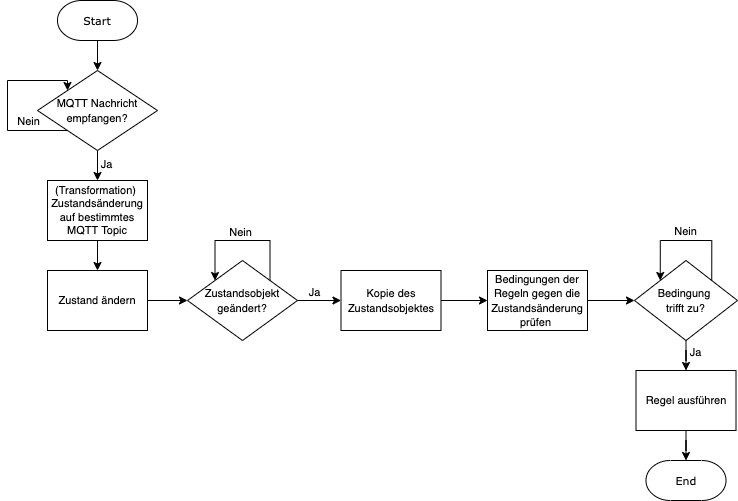
\includegraphics[width=14cm,height=11cm,keepaspectratio]{images/Programmablauf_Framework.png}
            \caption{Grober Programmablauf des Frameworks}
            \label{fig:programmablauf_framework}
        \end{figure}
        \\
        Aus dem Ablaufdiagramm gehen die parallele Ausführung von zwei voneinander unabhängigen Zustandsänderungen und die 
        erneute Änderung des Zustandes durch eine Regel selbst nicht hervor. Sofern die Änderungen unabhängig 
        sind, sollen Prozesse asynchron ablaufen, bzw. Regeln neue Zustandsänderungen hervorrufen können. 
        \\
        %\linebreak
        Zur Veranschaulichung hilft die nachfolgende Abbildung. 
        